\documentclass{beamer}


\usepackage{amsmath}
\usepackage[style=alphabetic,url=true]{biblatex}
\usepackage{environ}
\usepackage{geometry}
\usepackage{graphicx}
\usepackage{tikz}
\usepackage[T2A]{fontenc}
\usepackage[utf8]{inputenc}
\usepackage[cache=false]{minted}
\usepackage{amsmath}
\usepackage{amsfonts}
\usepackage{amssymb}
\usepackage{calrsfs}


% \usetheme{Bergen}

\usecolortheme{beaver}

\setbeamertemplate{itemize item}[circle]
\setbeamertemplate{itemize subitem}{--}
\addtobeamertemplate{navigation symbols}{}{
  \usebeamerfont{footline}%
  \usebeamercolor[fg]{footline}%
  \hspace{1em}%
  \insertframenumber/\inserttotalframenumber
}
\graphicspath{ {./graphics/} }
\setminted[Python]{
  fontsize=\tiny
}
\BeforeBeginEnvironment{minted}{\medskip}
\AfterEndEnvironment{minted}{\medskip}



\title{
  Біткоїн і криптовалютні технології \\
  Лекція 3: Основи криптографії 2/2
}

\author{Юрій Жикін}
\date{5 березня, 2024}

\begin{document}

\frame{\titlepage}

\begin{frame}
  \frametitle{Криптографія з публічним ключем: повторення}
  \begin{itemize}
  \item \textbf{Криптографічна система з публічним ключем} або \textbf{асиметрична
      криптографічна система} - це 
    криптографічна система, що використовує \textbf{пари} ключів:
    \begin{itemize}
    \item \textbf{приватний ключ}, який має зберігатись в таємниці власником,
    \item \textbf{публічний ключ}, який може бути публічно відомий всім.
    \end{itemize}
  \item Ключова ідея криптографії з публічним ключем - це те, що будь-хто, хто
    знає публічний ключ, може ``замкнути'' якусь інформацію цим ключем таким
    чином, що лише власник приватного ключа може ``відімкнути'' її.
  \item Відкрито Ральфом Мерклом, Вітфілдом Діффі, Мартіном Гелманом та іншими у
    1970-х.
  \item Чи не єдина причина, чому ми можемо робити хоч щось корисне в Інтернеті.
  \end{itemize}
\end{frame}

\begin{frame}
  \frametitle{Ідея обміну ключами Діффі-Гелмана-Меркла}
  \begin{itemize}
  \item Обмін ключами Діффі-Гелмана-Меркла інтуїтивно можна пояснити наступним
    прикладом:
  \end{itemize}
  \begin{center}
    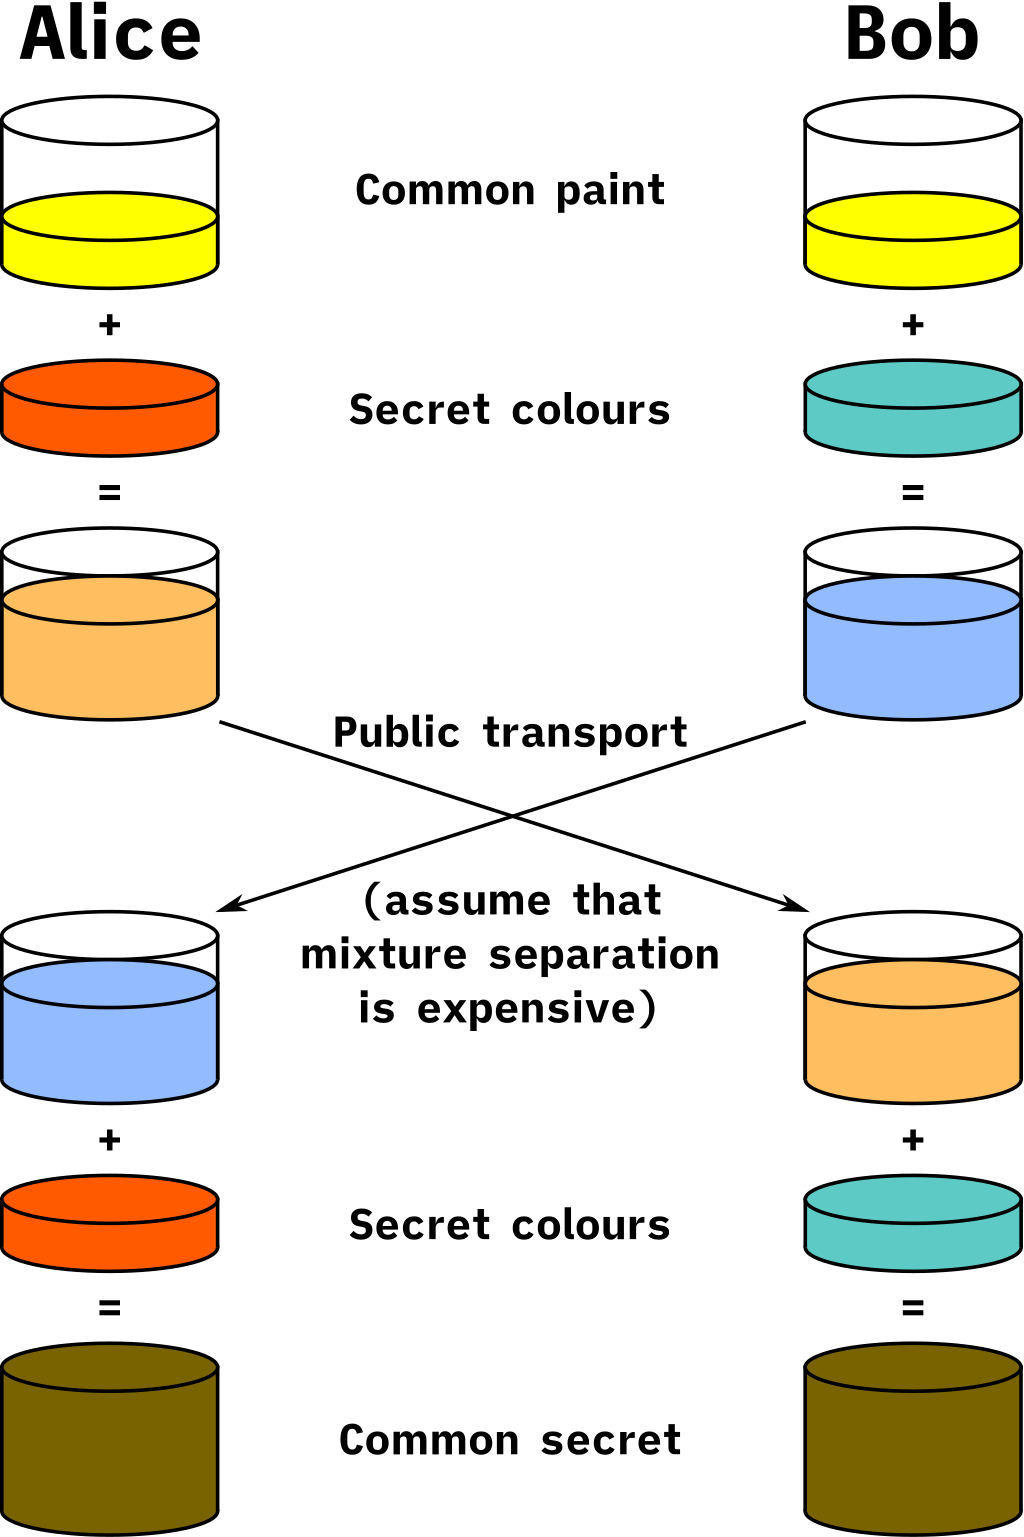
\includegraphics[width=0.35\textwidth]{dh}
  \end{center}
\end{frame}

\begin{frame}
  \frametitle{Поля 1/2}
  \begin{itemize}
  \item \textbf{Поле} - це множина елементів з визначеними операціями \textbf{додавання},
    \textbf{віднімання}, \textbf{множення} та \textbf{ділення}, що задовільняє
    \textbf{аксіоми поля}:
    \begin{small}
      \begin{align*}
        &\forall a, b, c: (a * b) * c = a * (b * c) \text{ -
          асоціативність для $+$ та $*$} \\
        &\forall a, b: a * b = b * a \text{ - комутативність для $+$ та
          $*$} \\
        &\exists e_+ = 0: \forall a: e + a = 0 + a = a \text{ - адитивна одиниця} \\
        &\exists e_* = 1: \forall a: e * a = 1 * a = a \text{ - мультиплікативна одиниця} \\
        &\forall a: \exists (-a): a + (-a) = e_+ = 0 \text{ - адитивна інверсія} \\
        &\forall a \neq 0: \exists (a^{-1}): a * (a^{-1}) = e_* = 1 \text{ -
          мультиплікативна інверсія} \\
        &\forall a, b, c: a*(b+c) = (a*b) + (a*c) \text{ - дистрибутивність $*$ над $+$} \\
      \end{align*}
    \end{small}
  \end{itemize}
\end{frame}

\begin{frame}
  \frametitle{Поля 2/2}
  \begin{itemize}
  \item Множина \textbf{раціональних чисел} $\mathbb{R}$ - це поле над
    звичайними операціями додавання та множення.
  \item В криптографії ми зазвичай розглядаємо \textbf{скінченні поля Галуа}
    \textbf{простого порядку} над операціями модульної арифметики:
    $$F_n = \mathbb{Z}/n\mathbb{Z} = {0, 1, ..., n - 1}$$
    де $n$ - це просте число; \textbf{така конструкція є полем тоді і тільки
      тоді, коли $n$ - просте число}.
  \end{itemize}
\end{frame}

\begin{frame}
  \frametitle{Групи 1/2}
  \begin{itemize}
  \item \textbf{Група} - це множина елементів з визначеною бінарною операцією,
    яка комбінує два елементи у третій елемент групи таким чином, що виконуються
    три \textbf{аксіоми групи}
    \begin{align*}
      &\forall a, b, c: (a \star b) \star c = a \star (b \star c) \text{ - асоціативність} \\
      &\exists e: \forall a: e \star a = a \text{ - існування одиниці} \\
      &\forall a: \exists b: a \star b = e \text{ - існування інверсії}
    \end{align*}
  \item \textbf{Породжуюча множина групи} - це підмножина елементів групи, така,
    що кожен елемент групи може бути представлений як комбінація скінченної
    кількості елементів цієї підмножини та їх обернених елементів.
  \item Група, що породжується одним елементом (який називається
    \textbf{генератором} і позначається літерою $G$), називається
    \textbf{циклічною}.
  \end{itemize}
\end{frame}

\begin{frame}
  \frametitle{Групи 2/2}
  \begin{itemize}
  \item Нехай $\mathbb{G}$ - це група. Нехай $a, b \in \mathbb{G}$. Позначимо
    операцію групи множенням, а її одиницю - 1. Нехай
    $$b^k = a$$
  \item $k$, яке задовільняє попереднє рівняння, називається \textbf{дискретним
      логаритмом} $a$ за основою $b$.
  \item Якщо ми позначимо операцію групи додаванням, а її одиницю - 0, позначення
    \textbf{дискретного логаритма} виглядатиме так
    $$kb = a$$
  \item \textbf{Задача пошуку дискретного логаритма} або \textbf{DLOG-задача}
    \textbf{вважається дуже складною для деяких груп}.
  \end{itemize}
\end{frame}

\begin{frame}
  \frametitle{Обмін ключами Діффі-Гелмана-Меркла 1/2}
  \begin{itemize}
  \item Реалізації протоколу ДГМ базуються на наступному спостереження,
    записаному адитивно
    \begin{align*}
      A &= aG (= G + G + ... + G) \\
      B &= bG \\
      bA &= b(aG) = (ba)G = (ab)G = a(bG) = aB
    \end{align*}
    або мультиплікативно
    \begin{align*}
      A &= G^a (= G * G * ... * G) \\
      B &= G^b \\
      A^b &= (G^a)^b = G^{(ab)} = G^{(ba)} = (G^b)^a = B^a
    \end{align*}
  \end{itemize}
\end{frame}

\begin{frame}
  \frametitle{Обмін ключами Діффі-Гелмана-Меркла 2/2}
  \begin{itemize}
  \item Найпростіша реалізація протоколу ДГМ (як описано у статті)
    використовує \textbf{мультиплікативну групу цілих чисел по модулю $p$}, де
    \textbf{$p$ - просте число}, а \textbf{ $g$ - примітивний корінь по модулю $p$}.
  \item Приклад ДГМ з малими числами:
    \begin{itemize}
      \scriptsize
    \item Еліс та Боб домовились використовувати числа по модулю $p = 23$ та
      основу $G = 5$.
    \item Еліс обирає таємне число $a = 4$ і надсилає Бобу
        $$A = G^a \pmod{p} = 5^4 \pmod{23} = 4$$
    \item Боб обирає таємне число $b = 3$ і надсилає Еліс
      $$B = G^b \pmod{p} = 5^3 \pmod{23} = 10$$
    \item Еліс обчислює
      $$s = B^a \pmod{p} = 10^4 \pmod{23} = 18$$
    \item Боб обчислює
      $$s = A^b \pmod{p} = 4^3 \pmod{23} = 18$$
    \end{itemize}
  \end{itemize}
\end{frame}

\begin{frame}
  \frametitle{Криптографічні підписи}
  \begin{itemize}
  \item \textbf{Схема криптографічних підписів} - це система для перевірки
    автентичності повідомлень.
  \item Схема криптографічних підписів складається з наступних трьох алгоритмів:
    \begin{itemize}
    \item алгоритм генерації ключів $Gen$, який обирає приватний ключ випадковим
      чином з множини всіх можливих приватних ключів,
    \item алгоритм підписування $Sign$, який, отримавши повідомлення та
      приватний ключ, створює підпис,
    \item алгоритм перевірки підпису $Verify$, який, отримавши повідомлення,
      публічний ключ та сам підпис, або приймає, або відкидає підпис.
    \end{itemize}
  \item Успішна перевірка підпису надає \textbf{дуже вагому} причину вірити, що
    дане повідомлення було автентифіковано власником відповідного приватного
    ключа.
  \end{itemize}
\end{frame}

\begin{frame}
  \frametitle{DSA 1/2}
  \begin{itemize}
  \item Еліс та Боб домовляються про параметри групи $(GROUP, G, n)$, де
    $GROUP$ - це група простого порядку $n$ з генератором $G$.
  \item Еліс створює пару ключів, що складається з приватного цілого числа $a$,
    випадково вибраного на проміжку $[1, n - 1]$ та публічного елемента групи
    $A = aG$.
  \item Для того, щоб підписати повідомлення $m$, Еліс
    \begin{itemize}
    \item обчислює $e = HASH(m)$,
    \item обирає \textbf{криптографічно безпечне випадкове ціле число}
      $k \in [1, n - 1]$,
    \item обчислює елемент групи $x = kG$,
    \item обчислює $r = x \pmod{n}$,
    \item обчислює $s = k^{-1}(e + ra) \pmod{n}$.
    \end{itemize}
  \item Підпис - це пара значень $(r, s)$; $(r, -s \pmod{n})$ - \textbf{також
      правильний підпис}.
  \end{itemize}
\end{frame}

\begin{frame}
  \frametitle{DSA 2/2}
  \begin{itemize}
  \item Для перевірки підпису $(r, s)$ Боб
    \begin{itemize}
    \item перевіряє, що $r$ та $s$ є цілими числами в проміжку $[1, n - 1]$,
      інакше підпис недійсний,
    \item обчислює $e = HASH(m)$,
    \item обчислює $u_1 = es^{-1} \pmod{n}$ та $u_2 = rs^{-1} \pmod{n}$,
    \item обчислює елемент групи $x = u_1G + u_2A$.
    \end{itemize}
  \item Підпис дійсний, якщо $r \equiv x_1 \pmod{n}$ та недійсний у протилежному
    випадку:
    \begin{align*}
      u_1G + u_2A &= u_1G + u_2aG = (u_1 + u_2a)G \\
                  &= (es^{-1} + rs^{-1}a)G = (e + ra)s^{-1}G \\
                  &= (e + ra)(a + ra)^{-1}kG = kG \\
                  &= r
    \end{align*}
  \end{itemize}
\end{frame}

\begin{frame}
  \frametitle{ECDSA}
  \begin{itemize}  
  \item З DSA, бітовий розмір ключа, що дає бажаний рівень безпеки, становить
    2048 або навіть 3072 бітів.
  \item З \textbf{еліптичними кривими}, бітовий розмір приватного ключа, який
    вважається достатнім для \textbf{ECDSA}, приблизно \textbf{вдвічі більший}
    за бажаний рівень безпеки, тобто для отримання 128 бітів безпеки достатньо
    ключа розміром 256 бітів.
  \item \textbf{Алгоритм цифрових підписів на еліптичній кривій}
    (\textbf{Elliptic Curve Digital Signature Algorithm, ECDSA}) - це варіант
    алгоритму \textbf{DSA}, який використовує групу еліптичної кривої замість
    мультиплікативної групи.
  \end{itemize}
\end{frame}

\begin{frame}
  \frametitle{Еліптичні криві 1/3}
  \begin{itemize}
  \item \textbf{Еліптичні криві} - це алгебраїчні структури, що описуються
    рівняннями, які мають форму:
    $$y^2 = x^3 + ax + b$$
  \end{itemize}
  \begin{center}
    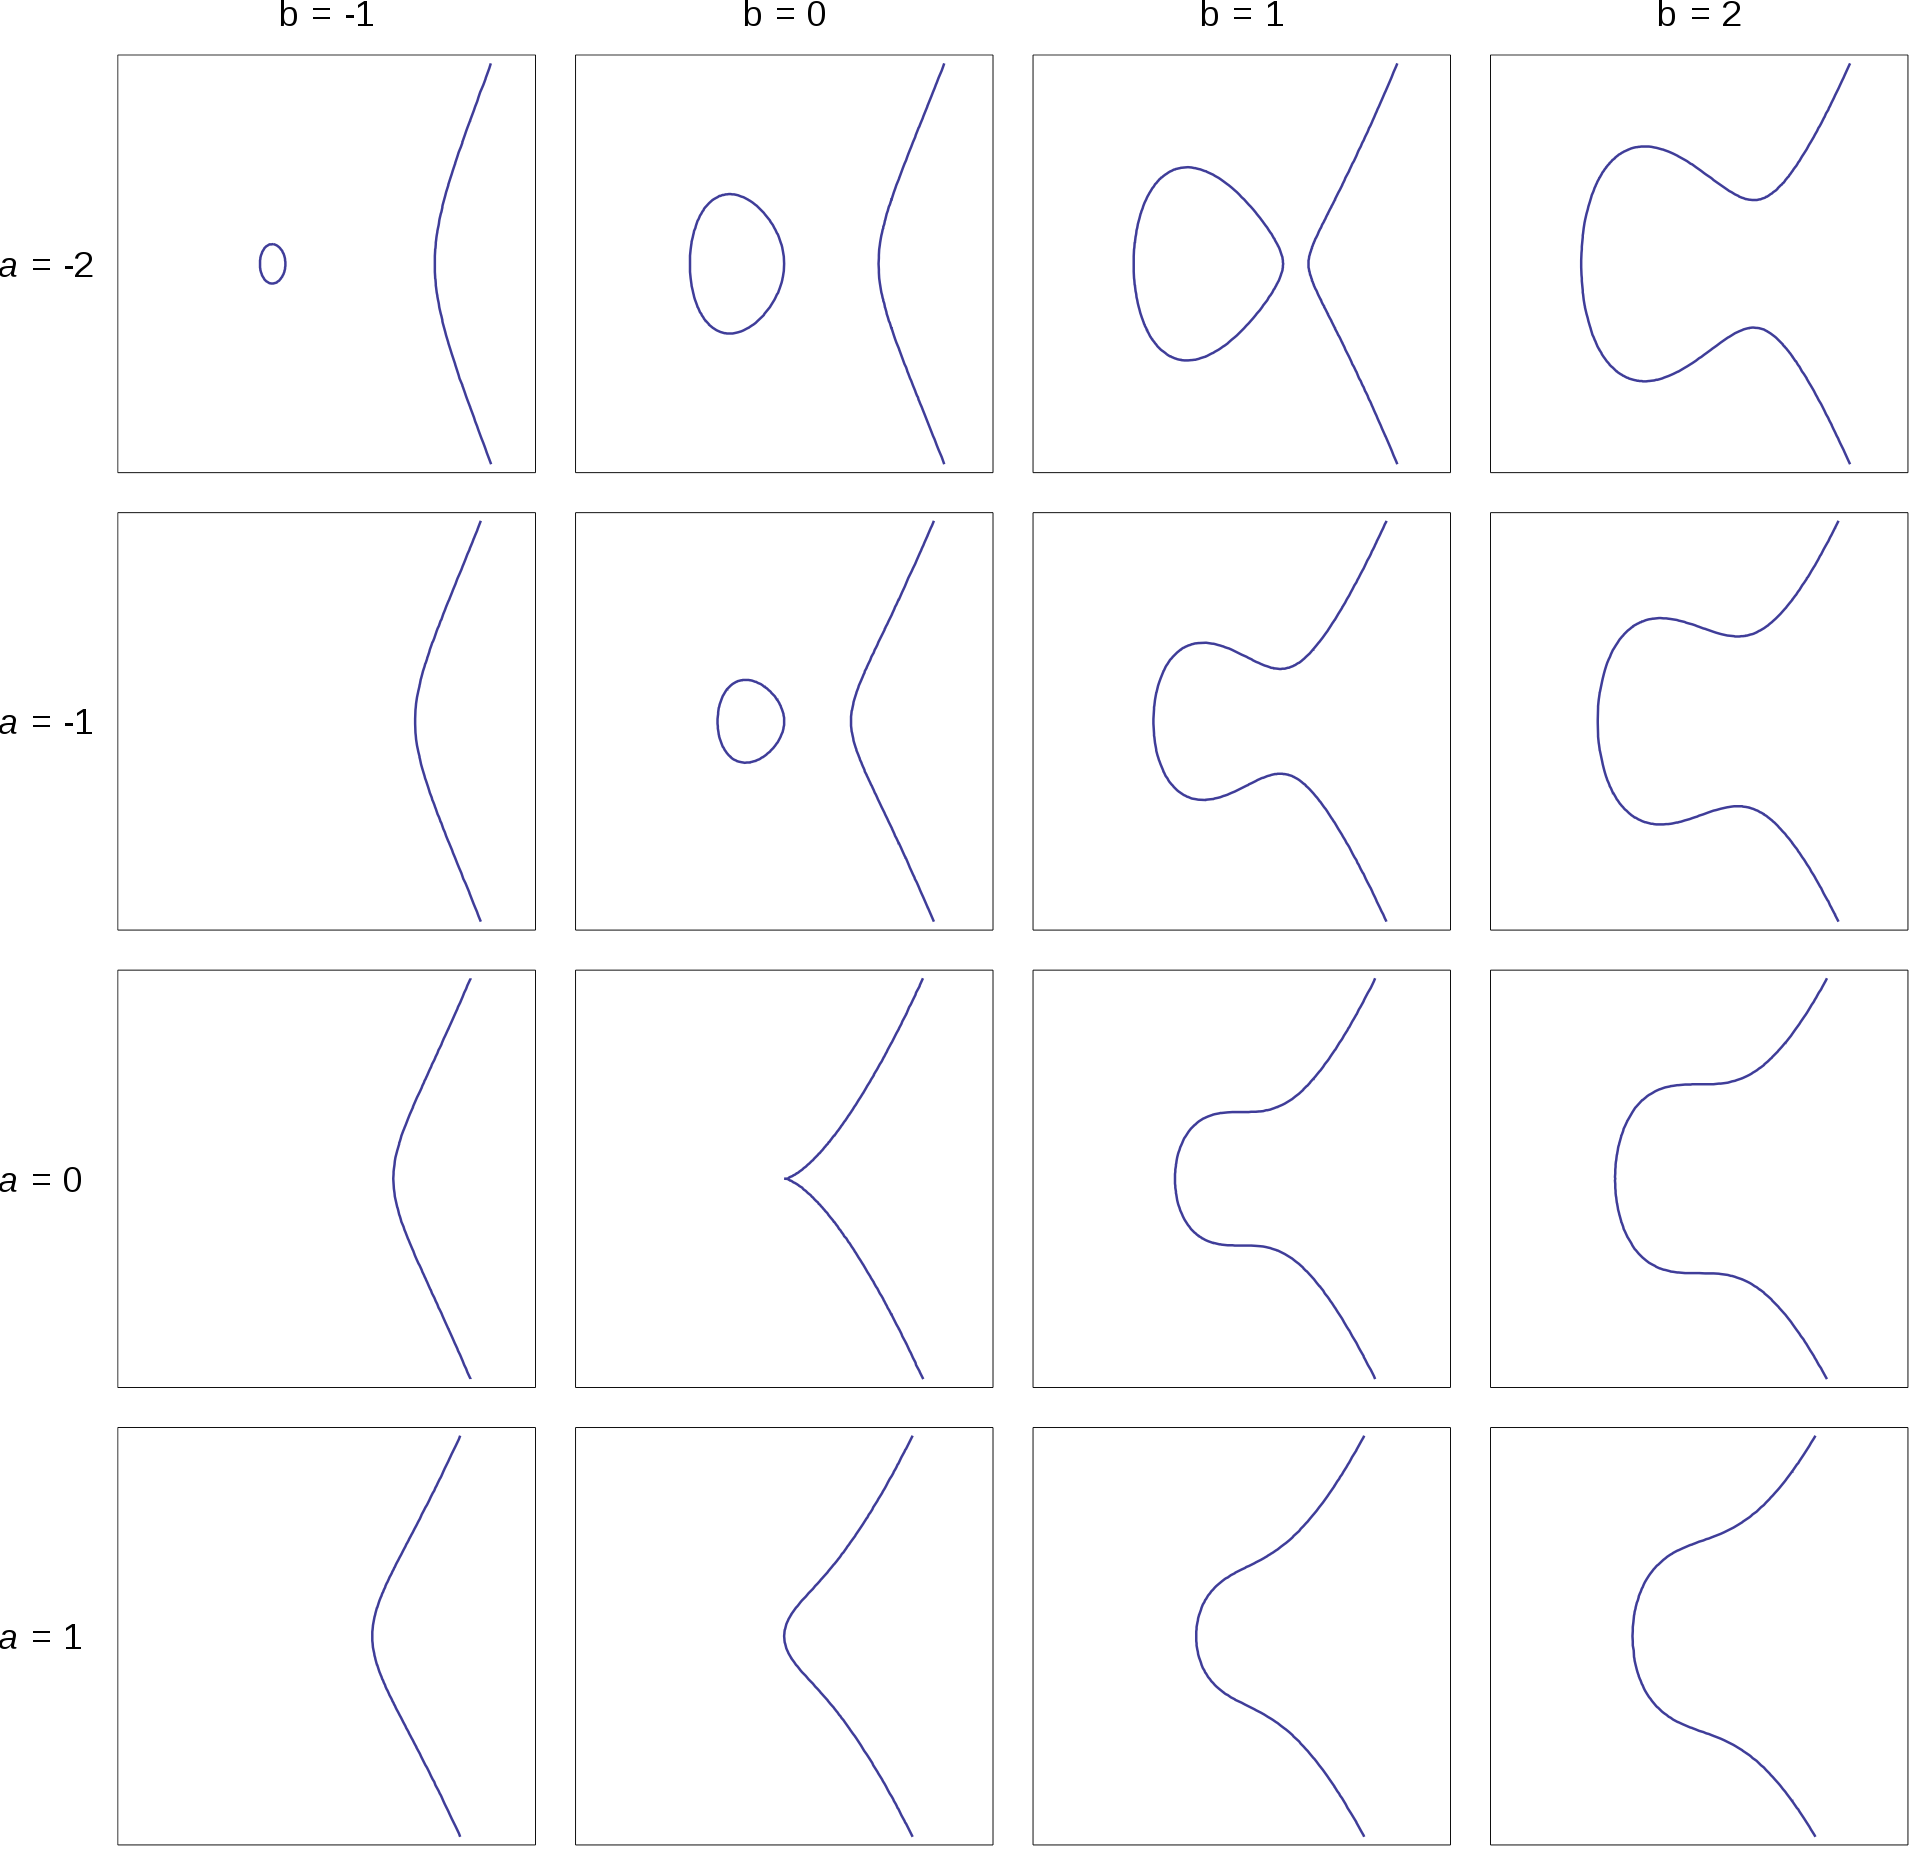
\includegraphics[width=0.55\textwidth]{ec}
  \end{center}
\end{frame}

\begin{frame}
  \frametitle{Еліптичні криві 2/3}
  \begin{itemize}
  \item Еліптична крива, визначена над \textbf{полем} $K$, складається з точок в
    множині $K \times K$ і утворює \textbf{групу}.
  \item \textbf{Груповий закон}:
    \begin{itemize}
    \item Якщо $P$ та $Q$ - дві точки кривої, тоді ми можемо однозначно описати
      третю точку кривої, $P + Q$, наступним чином. Спочатку, будуємо пряму, що
      перетинає криву у точках $P$ та $Q$, яка в загальному випадку перетинає
      криву у ще одній точці, $R$. Тоді встановлюємо, що $P + Q$ - це точка
      $-R$, протилежна точці $R$ відносно осі $x$.
    \end{itemize}
  \end{itemize}
  \begin{center}
    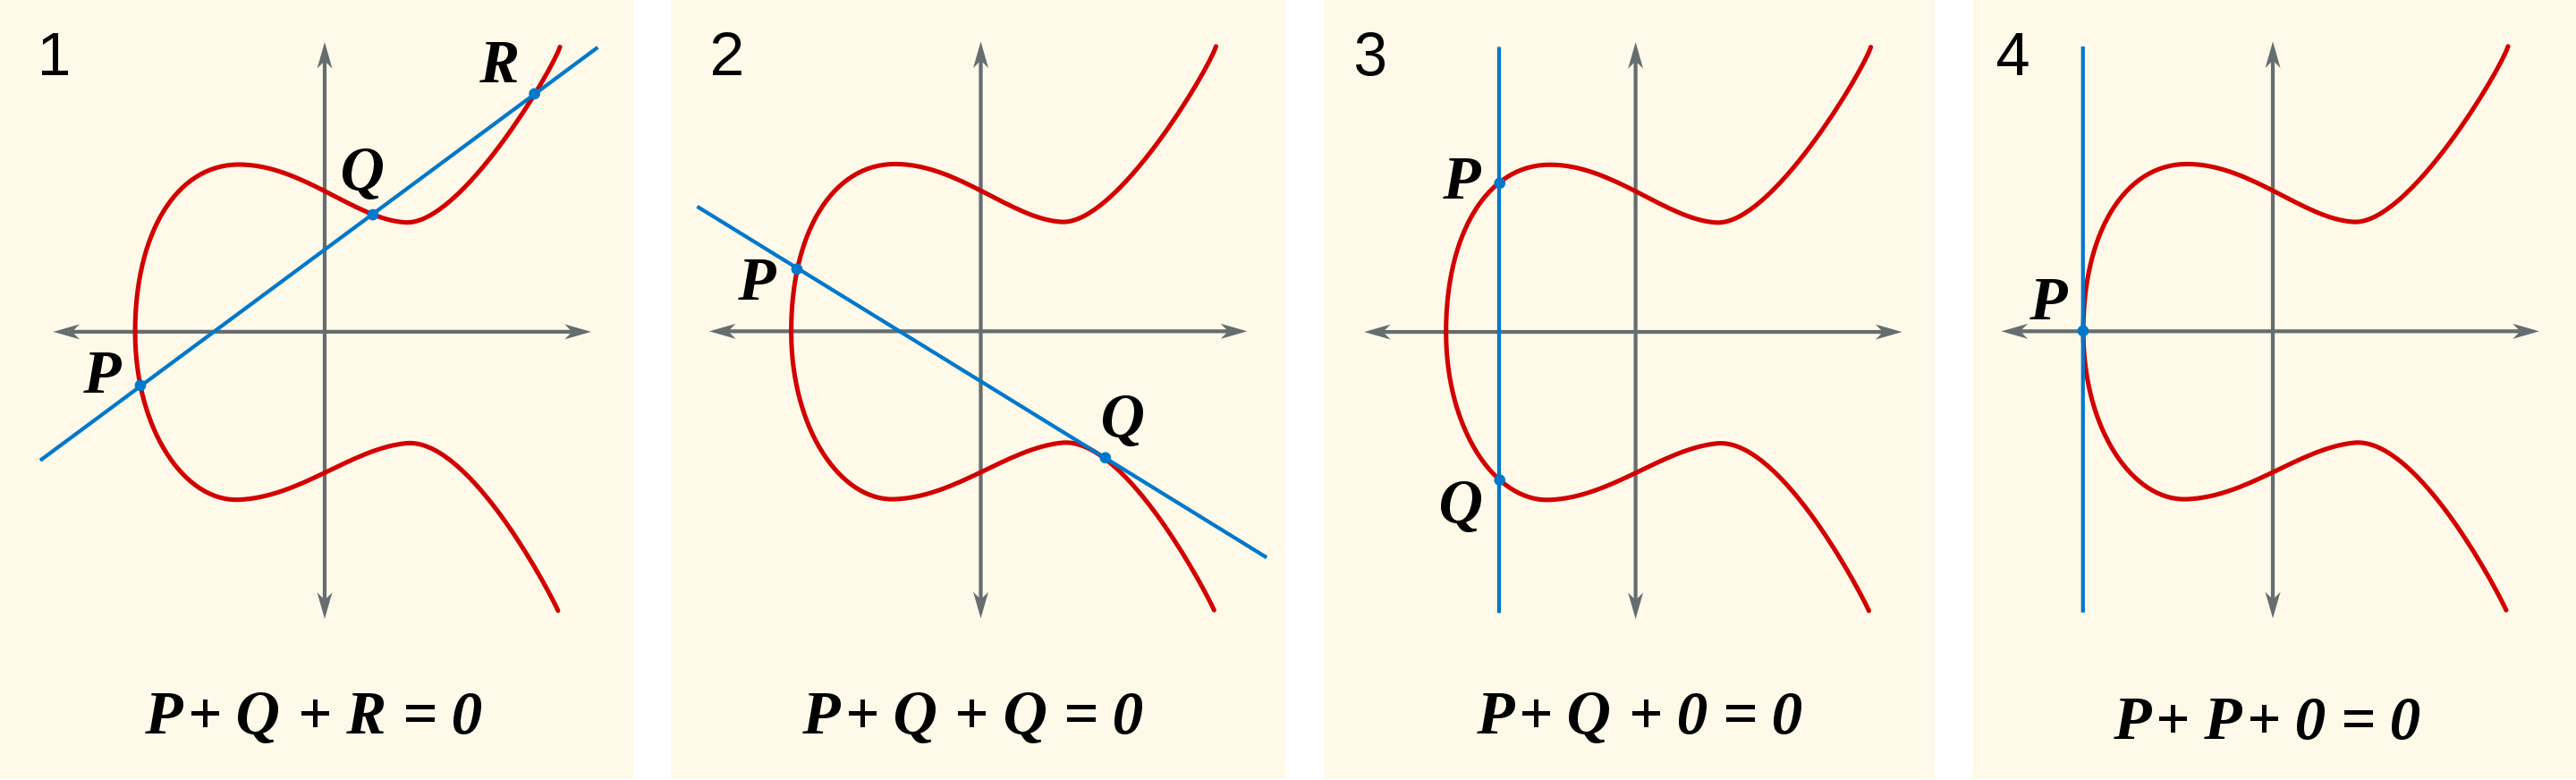
\includegraphics[width=0.9\textwidth]{ec_group}
  \end{center}
\end{frame}

\begin{frame}
  \frametitle{Еліптичні криві 3/3}
  \begin{itemize}
  \item \textbf{Еліптичні криві, визначені над скінченними полями простих
      порядків}, утворюють групи, що мають значно складнішу алгебраїчну
    структуру, і тому добре підходять для використання у криптографії, бо
    дозволяють використовувати значно \textbf{менші ключі}.
  \item Приклад еліптичної кривої, визначеної над скінченним полем ($y^2 = x
    ^3 - x$ над $F_{71}$):
  \end{itemize}
  \begin{center}
    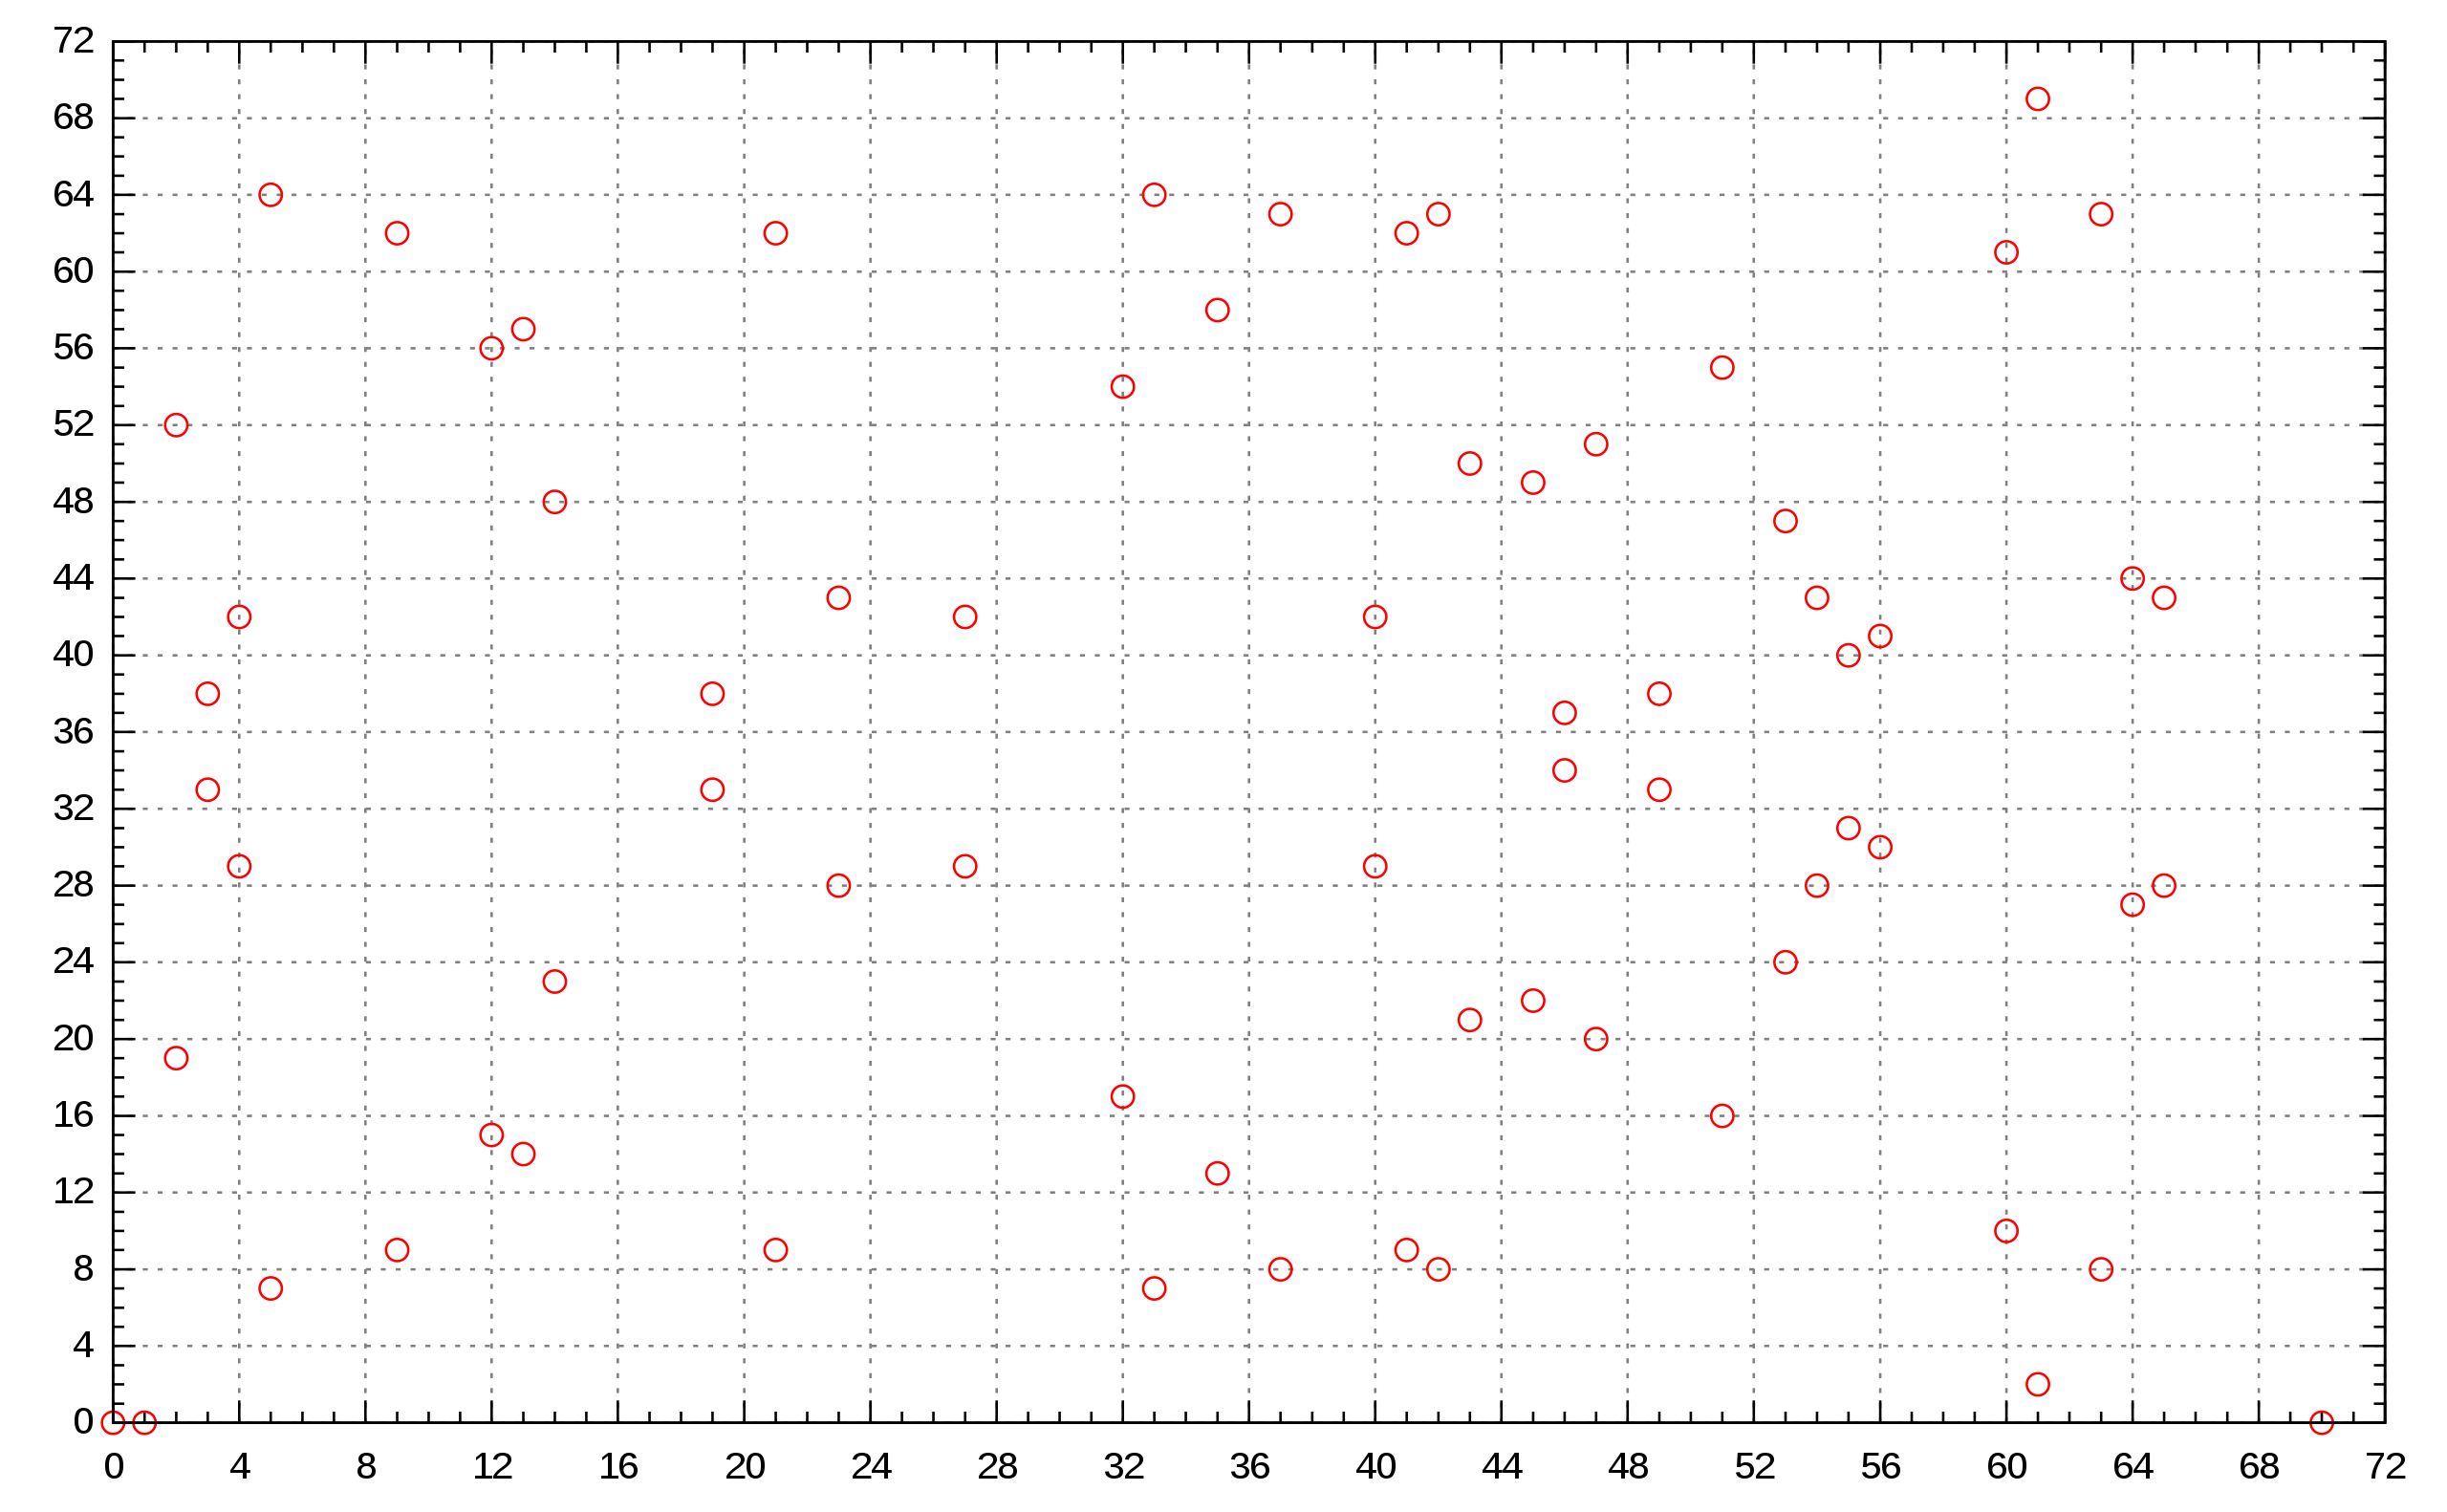
\includegraphics[width=0.7\textwidth]{ec_finite_field_group}
  \end{center}
\end{frame}

\begin{frame}
  \frametitle{Еліптична крива SECP256K1 1/2}
  \begin{itemize}
  \item Еліптична крива, що використовується у Біткоїні для підписування
    транзакцій, називається \textbf{secp256k1}.
  \item Ця еліптична крива визначена над скінченним полем $F_p$, де
    $$p = 2^{256} - 2^{32} - 2^9 - 2^8 - 2^7 - 2^6 - 2^4 - 1$$ і описується рівнянням
    $$y^2 = x^3 + 7$$
  \end{itemize}
  \begin{center}
    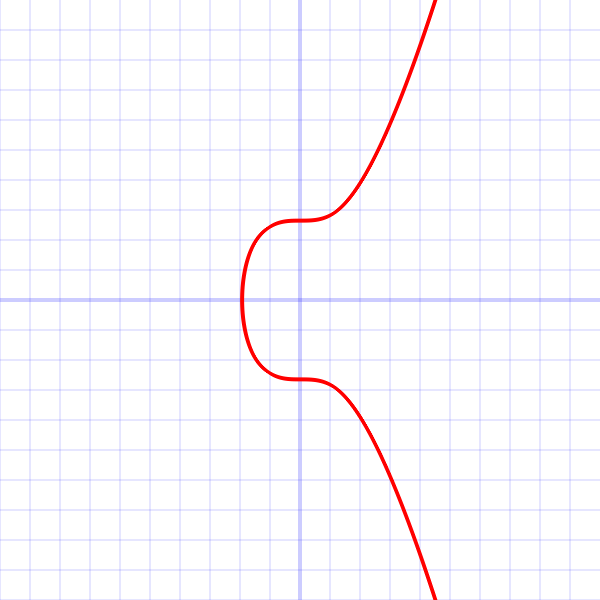
\includegraphics[width=0.3\textwidth]{secp256k1}
  \end{center}
\end{frame}

\begin{frame}
  \frametitle{Еліптична крива SECP256K1 2/2}
  \begin{small}
    \begin{itemize}
    \item Крива \textbf{secp256k1} побудована спеціальним невипадковим чином, що
      дозволяє використовувати високошвидкісну реалізацію операцій.
    \item На відміну від криптографічних кривих, що рекомендуються NIST, за
      винятком кривої \textbf{curve25519}), константи кривої \textbf{secp256k1}
      обрані передбачуваним чином, що значно зменшує ймовірність того, що в ній є
      ``задні двері''.
    \item \textbf{libsecp256k1} - це високооптимізована реалізація кривої
      \textbf{secp256k1}, що була виділена з бази коду проєкту Bitcoin Core в
      окремий проєкт:
      \begin{center}
        https://github.com/bitcoin-core/secp256k1
      \end{center}
    \item Біткоїн використовує \textbf{secp256k1} як для традиційних підписів
      ECDSA, так і для підписів Шнора, які були впроваджені в рамках зміни проколу
      під назвою \textbf{Taproot} (англ. ``стрижневий корінь''), яка була
      активована 14 листопада 2021 року.
    \end{itemize}
  \end{small}
\end{frame}

\begin{frame}
  \frametitle{Корисні ресурси}
  \begin{itemize}
  \item \textbf{A Computational Introduction to Number Theory and Algebra} by
    Victor Shoup
    \begin{itemize}
    \item https://shoup.net/ntb/
    \end{itemize}
  \end{itemize}
\end{frame}

\begin{frame}
  \frametitle{Кінець}
  \begin{center}
    Дякую за увагу!
  \end{center}
\end{frame}

\end{document}

%%% Local Variables:
%%% mode: latex
%%% TeX-master: t
%%% End:
